\documentclass{article}
\usepackage{graphicx} % Required for inserting images
\usepackage{enumitem}
\usepackage{xcolor}
\usepackage{listings}
\usepackage{mathtools}
\usepackage{amsmath}
\newcommand{\logicarg}[2]{% \logicarg{<premise>}{<conclusion>}
  \begin{tabular}[t]{@{}l@{}}
    #1 \\ \hline #2
  \end{tabular}%
}

\setlength{\oddsidemargin}{-0.25in}
\setlength{\topmargin}{-0.5in}
\setlength{\headheight}{0cm}
\setlength{\headsep}{0cm}
\setlength{\textheight}{10in}
\setlength{\textwidth}{7in}
\setlength{\topskip}{0cm}

\begin{document}

\noindent\textbf{ComS 472 - PS8 \quad Due: Nov 10, 2024 \quad Name: Aren Ashlock}

\begin{enumerate}

% ------------------------------------- 1 DONE -------------------------------------

\item \textbf{(22 pts)} (Exercise 9.29) Here are two sentences in the language of first-order logic:

\begin{equation*}
    \text{(A)} \quad \forall x \exists y \text{ } x \geq y
\end{equation*}
\begin{equation*}
    \text{(B)} \quad \exists y \forall x \text{ } x \geq y
\end{equation*}

Assume that the variables range over all the natural numbers 0, 1, 2, ..., and that the “$\geq$” predicate means “is greater than or equal to.”

    \begin{enumerate}[label=($\alph*$)]

    % ----------------------------------- 1a DONE -----------------------------------

    \item \textbf{(3 pts)} Translate (A) and (B) into English.

    \color{blue}
        (A) For all natural numbers, there exists a natural number that is less than or equal to it.\\
        (B) There exists a natural number that is less than or equal to all other natural numbers.
    \color{black}

    % -------------------------------------------------------------------------------

    % ----------------------------------- 1b DONE -----------------------------------

    \item \textbf{(2 pts)} Is (A) true under this interpretation?

    \color{blue}
        Yes
    \color{black}

    % -------------------------------------------------------------------------------

    % ----------------------------------- 1c DONE -----------------------------------

    \item \textbf{(2 pts)} Is (B) true under this interpretation?

    \color{blue}
        Yes
    \color{black}

    % -------------------------------------------------------------------------------

    % ----------------------------------- 1d DONE -----------------------------------

    \item \textbf{(2 pts)} Does (A) logically entail (B)?

    \color{blue}
        No
    \color{black}

    % -------------------------------------------------------------------------------

    % ----------------------------------- 1e DONE -----------------------------------

    \item \textbf{(2 pts)} Does (B) logically entail (A)?

    \color{blue}
        Yes
    \color{black}

    % -------------------------------------------------------------------------------

    % ----------------------------------- 1f DONE -----------------------------------

    \item \textbf{(5 pts)} Using resolution, try to prove that (A) follows from (B). Do this even if you think that (B) does not logically entail (A); continue until the proof breaks down and you cannot proceed (if it does break down). Show the unifying substitution for each resolution step. If the proof fails, explain exactly where, how, and why it breaks down.

    \color{blue}
        To show (A) follows from (B), we need to prove $B \models A$, which means we need to derive an empty clause from $B \wedge \neg A$.\\
        $B$: $\exists y \forall x$ $x \geq y$ can be written as $(x \geq a)$ using skolemization.\\
        $\neg A$: $\neg (\forall x \exists y$ $x \geq y)$, which is $\exists x \forall y$ $\neg(x \geq y)$. Using skolemization, we get $\neg (b \geq y)$.\\
        These unify under $\{a/y, b/x\}$.\\
        Then, using resolution, we get an empty clause.\\
        Thus, the proof is successful showing a contradiction and that (A) \textbf{DOES }follow from (B).
    \color{black}

    % -------------------------------------------------------------------------------

    % ----------------------------------- 1g DONE -----------------------------------

    \item \textbf{(6 pts)} Now try to prove that (B) follows from (A).

    \color{blue}
        To show (B) follows from (A), we need to prove $A \models B$, which means we need to derive an empty clause from $A \wedge \neg B$.\\
        $A$: $\forall x \exists y$ $x \geq y$ can be written as $(x \geq C(x))$ using a skolemization function since y depends on x.\\
        $\neg B$: $\neg (\exists y \forall x$ $x \geq y)$, which is $\forall y \exists x$ $\neg(x \geq y)$. Using a skolemization function (since x depends on y), we get $\neg (D(y) \geq y)$.\\
        There is no possible unification, so the proof breaks down and shows that (B) \textbf{DOES NOT }follow from (A).
    \color{black}

    % -------------------------------------------------------------------------------
    
    \end{enumerate}

% ----------------------------------------------------------------------------------

% ------------------------------------- 2 DONE -------------------------------------

\item \textbf{(6 pts)} A slot machine is rigged so you get -1, 0, or 1 with equal probability on the first spin $X$. On the second spin $Y$ you get 1 if $X$ = 0, and 0 if $X \neq$ 0. The two random variables are dependent because the realization of $Y$ depends on the realization of $X$. Compute the expected values $E(X)$, $E(Y)$, and $E(XY)$.

\color{blue}
    $E(X) = (1)(\frac{1}{3}) + (0)(\frac{1}{3}) + (-1)(\frac{1}{3}) = 0$\\
    $E(Y) = (1)(\frac{1}{3}) + (0)(\frac{2}{3}) = \frac{1}{3}$\\
    $E(XY) = (0)(\frac{1}{3}) + (0)(\frac{1}{3}) + (0)(\frac{1}{3}) = 0$
\color{black}

% ----------------------------------------------------------------------------------

% ------------------------------------- 3 DONE -------------------------------------

\item \textbf{(9 pts)} (Exercise 13.3) For each of the following statements, either prove it is true or give a counterexample.

    \begin{enumerate}[label=($\alph*$)]

    % ----------------------------------- 3a DONE -----------------------------------

    \item \textbf{(3 pts)} If $P(a$ $|$ $b,c) = P(b$ $|$ $a,c)$, then $P(a$ $|$ $c) = P(b$ $|$ $c)$.

    \color{blue}
        This is \textbf{TRUE}\\
        The first part is: $\frac{P(a \wedge b \wedge c)}{P(b \wedge c)} = \frac{P(b \wedge a \wedge c)}{P(a \wedge c)}$. This is true when $P(b \wedge c) = P(a \wedge c)$.\\
        Looking at the second part: $\frac{P(a \wedge c)}{P(c)} = \frac{P(b \wedge c)}{P(c)}$. This also results in true when $P(b \wedge c) = P(a \wedge c)$.\\
        Thus, $True \Rightarrow True$ means the statement is true.
    \color{black}

    % -------------------------------------------------------------------------------

    % ----------------------------------- 3b DONE -----------------------------------

    \item \textbf{(3 pts)} If $P(a$ $|$ $b,c) = P(a)$, then $P(b$ $|$ $c) = P(b)$.

    \color{blue}
        This is \textbf{FALSE}\\
        Use the following probabilities: $P(a)=0.2, P(b)=0.5, P(c)=0.3$\\
        The first part of the statement evaluates to: $\frac{P(a \wedge b \wedge c)}{P(b \wedge c)} = P(a)$. Plugging in the values gets $\frac{0.2(0.5)(0.3)}{0.5(0.3)} = 0.2$, which algebra reduces it down to $0.2 = 0.2$. This is true.\\
        As for the second part: $0.5(0.3) = 0.2(0.3)$, which $0.15 = 0.06$ is false.\\
        Since we get $True \Rightarrow False$, the entire statement is false.
    \color{black}

    % -------------------------------------------------------------------------------

    % ----------------------------------- 3c DONE -----------------------------------

    \item \textbf{(3 pts)} If $P(a$ $|$ $b) = P(a)$, then $P(a$ $|$ $b,c) = P(a$ $|$ $c)$.

    \color{blue}
        This is \textbf{TRUE} (assuming the probabilities are independent of each other)\\
        The first part is: $\frac{P(a \wedge b)}{P(b)} = P(a)$, which can be written as $\frac{P(a)P(b)}{P(b)} = P(a)$, which is also $P(a) = P(a)$. This is always true.\\
        Looking at the second part: $\frac{P(a \wedge b \wedge c)}{P(b \wedge c)} = \frac{P(a \wedge c)}{P(c)}$, which can be written as $\frac{P(a)P(b)P(c)}{P(b)P(c)} = \frac{P(a)P(c)}{P(c)}$, which is also $P(a) = P(a)$. This is always true.\\
        Thus, $True \Rightarrow True$ means the statement is true.
    \color{black}

    % -------------------------------------------------------------------------------
    
    \end{enumerate}

% ----------------------------------------------------------------------------------

% ------------------------------------- 4 DONE -------------------------------------

\item \textbf{(13 pts)} (Exercise 13.8) You are given the full joint distribution below.

\begin{center}
    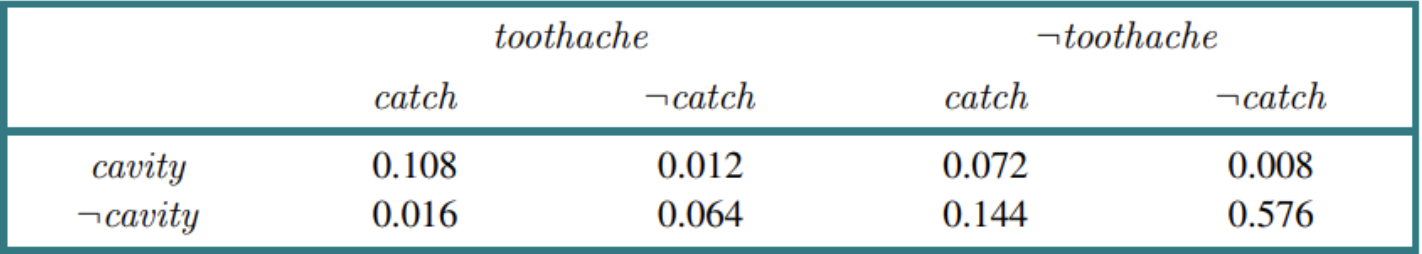
\includegraphics[scale=0.6]{472-PS8-Q4.png}
\end{center}

Calculate the following probability distributions:

    \begin{enumerate}[label=($\alph*$)]

    % ----------------------------------- 4a DONE -----------------------------------

    \item \textbf{(3 pts)} $\mathbf{P}(Toothache)$.

    \color{blue}
        $0.108 + 0.012 + 0.016 + 0.064 = 0.2$\\
        $\mathbf{P}(Toothache) = \langle 0.2, 0.8 \rangle$
    \color{black}

    % -------------------------------------------------------------------------------

    % ----------------------------------- 4b DONE -----------------------------------

    \item \textbf{(3 pts)} $\mathbf{P}(Cavity)$.

    \color{blue}
        $0.108 + 0.012 + 0.072 + 0.008 = 0.2$\\
        $\mathbf{P}(Cavity) = \langle 0.2, 0.8 \rangle$
    \color{black}

    % -------------------------------------------------------------------------------

    % ----------------------------------- 4c DONE -----------------------------------

    \item \textbf{(3 pts)} $\mathbf{P}(Toothache$ $|$ $cavity)$.

    \color{blue}
        $\frac{\mathbf{P}(Toothache \wedge cavity)}{\mathbf{P}(cavity)} = \frac{0.108 + 0.012}{0.2} = \frac{0.12}{0.2} = 0.6$\\
        $\mathbf{P}(Toothache$ $|$ $cavity) = \langle 0.6, 0.4 \rangle$
    \color{black}

    % -------------------------------------------------------------------------------

    % ----------------------------------- 4d DONE -----------------------------------

    \item \textbf{(4 pts)} $\mathbf{P}(Cavity$ $|$ $toothache$ $\vee$ $catch)$.

    \color{blue}
        $\frac{\mathbf{P}(Cavity \wedge (toothache \vee catch)}{\mathbf{P}(toothache \vee catch)} = \frac{0.108 + 0.012 + 0.072}{0.108 + 0.012 + 0.016 + 0.064 + 0.072 + 0.144} = \frac{0.192}{0.416} \approx 0.462$\\
        $\mathbf{P}(Cavity$ $|$ $toothache$ $\vee$ $catch) = \langle 0.462, 0.538 \rangle$
    \color{black}

    % -------------------------------------------------------------------------------
    
    \end{enumerate}

% ----------------------------------------------------------------------------------

\end{enumerate}
\end{document}